
%%%%%%%%%%%%%%%%% Introduction to the Assignment %%%

In this Assignment, \textit{\textbf{Problem 5 - Optimization of phased array antenna radiation pattern and array configuration}}, a phased array consisting of 64 lined up isotropic antennas shall be configured and its configuration investigated. The antenna beam shall be a composite vertical beam in vertical direction, with a operating frequency of 53 MHz.

The design shall be done according to the given equation \ref{eq:orig} in Röttger, chap. 2.1 \citep{roettger1989instrumental}.

\begin{equation}
	E(\delta) = \sum_{n=1}^N E_n(\delta) \exp \Bigg(i\Big(\sin(\delta)\frac{2 \pi (n-1)d}{\lambda}  + \varphi_n \Big)\Bigg)
	\label{eq:orig}
\end{equation}

Additionally, the variables of the design shall be investigated and proper values found.

%%%%%%%%%%%%%%%%% TASK intro %%%
\section{Array Factor Derivation}
To understand the different implications of the variables of the given equation \ref{eq:orig}, it is helpful to derive the equation. Also one should take into account the pattern multiplication theorem \citep{donohoe:lecture}, where the array pattern is given as product of each array element pattern times the array factor (AF).
Based on the given boundary condition to use an isotropic radiator (located at origin), the initial equation to start with is the one for the (far) field of an isotropic radiator

\begin{equation}
	E = I_0 \frac{e^{-jkr}}{4\pi r}
	\label{eq:iso_radiator}
\end{equation}
with $I_0$ as current on the antenna, $k$ as wavenumber given by $k = \frac{2\pi}{\lambda}$ and $r$ the distance to the target.
Assuming that the current magnitudes of the array elements are equal, and using the first (origin) array element as phase reference, means this array element has $\varphi = 0$ \citep{donohoe:lecture}, the currents on the array elements are as follows:

\begin{equation}
	I_1 = I_0 , \quad I_2 = I_0 \exp(j \varphi_{2}), \quad \dots \quad I_N = I_o \exp(j \varphi_{N})
	\label{eq:currents}
\end{equation}
with $N$ being the number of array elements.

The distance to the target for each array element can be easily derived using simple geometry (c.f. fig. \ref{fig:radiationPattern}).

\begin{figure}[!h]
\centering
	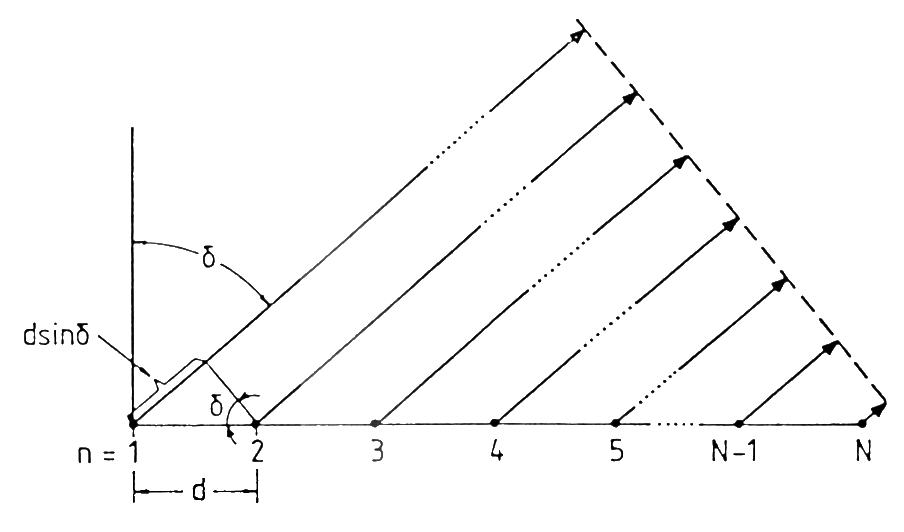
\includegraphics[width=0.7\textwidth]{images/PAradiationPattern}
	\caption{Wave vectors radiated from isotropic antenna elements with spacing d under zenith angle $\delta$ \citep[c.f.][Figure 10]{roettger1989instrumental}}
	\label{fig:radiationPattern}
\end{figure}

Combining the different distances to the targets with the appropriate current for each array element and inserting it into equation \ref{eq:iso_radiator} leads to the radiation pattern for each antenna, denoted in eq. \ref{eq:fieldsOfArray}. 

\begin{equation}
\begin{split}
	E_1(\delta) \approx I_0 \frac{e^{-jkr}}{4\pi r}\\
	\vdots \\
	E_N(\delta) \approx I_0 \exp(j\varphi_{N}) \frac{\exp(-jk\[r - (N-1)d\sin\delta\])}{4\pi r}
\end{split}
\end{equation}

Assuming that all antennas are the same and have the same pattern, the fields

%%%%%%%%%%%%%%%%% TASK 1 %%%
\section{Optimal distance between array elements}



%%%%%%%%%%%%%%%%% TASK 2 %%%
\section{Number of antenna elements}


%%%%%%%%%%%%%%%%% TASK 3 %%%
\section{Spatial Weighting}


%%%%%%%%%%%%%%%%% TASK 4 %%%
\section{Optimal Design for antenna array}


%%%%%%%%%%%%%%%%% TASK 5 %%%
\section{Main lobe maximum and width}


%%%%%%%%%%%%%%%%% TASK 6 %%%
\section{Radiation pattern change when non-vertical beam}


%%%%%%%%%%%%%%%%% TASK 7 %%%
\section{Electrical Weighting}
